\subsubsection{Data Path} 
The design of the fitness core is highly influenced by the classic pipelined MIPS core design\cn.
The core is designed as a five stage pipeline.
The contents of the different stages in the pipeline, however, differs from the original MIPS architecture, as the CPU architecture has to accomadate for the ISA design which combines ideas from multiple exisiting architectures.
An overview of the data path can be seen in figure \vref{fpga:fig:fitness:fitness_arch}

\begin{figure}

  \centering
  % Trim er [left bottom right top]
  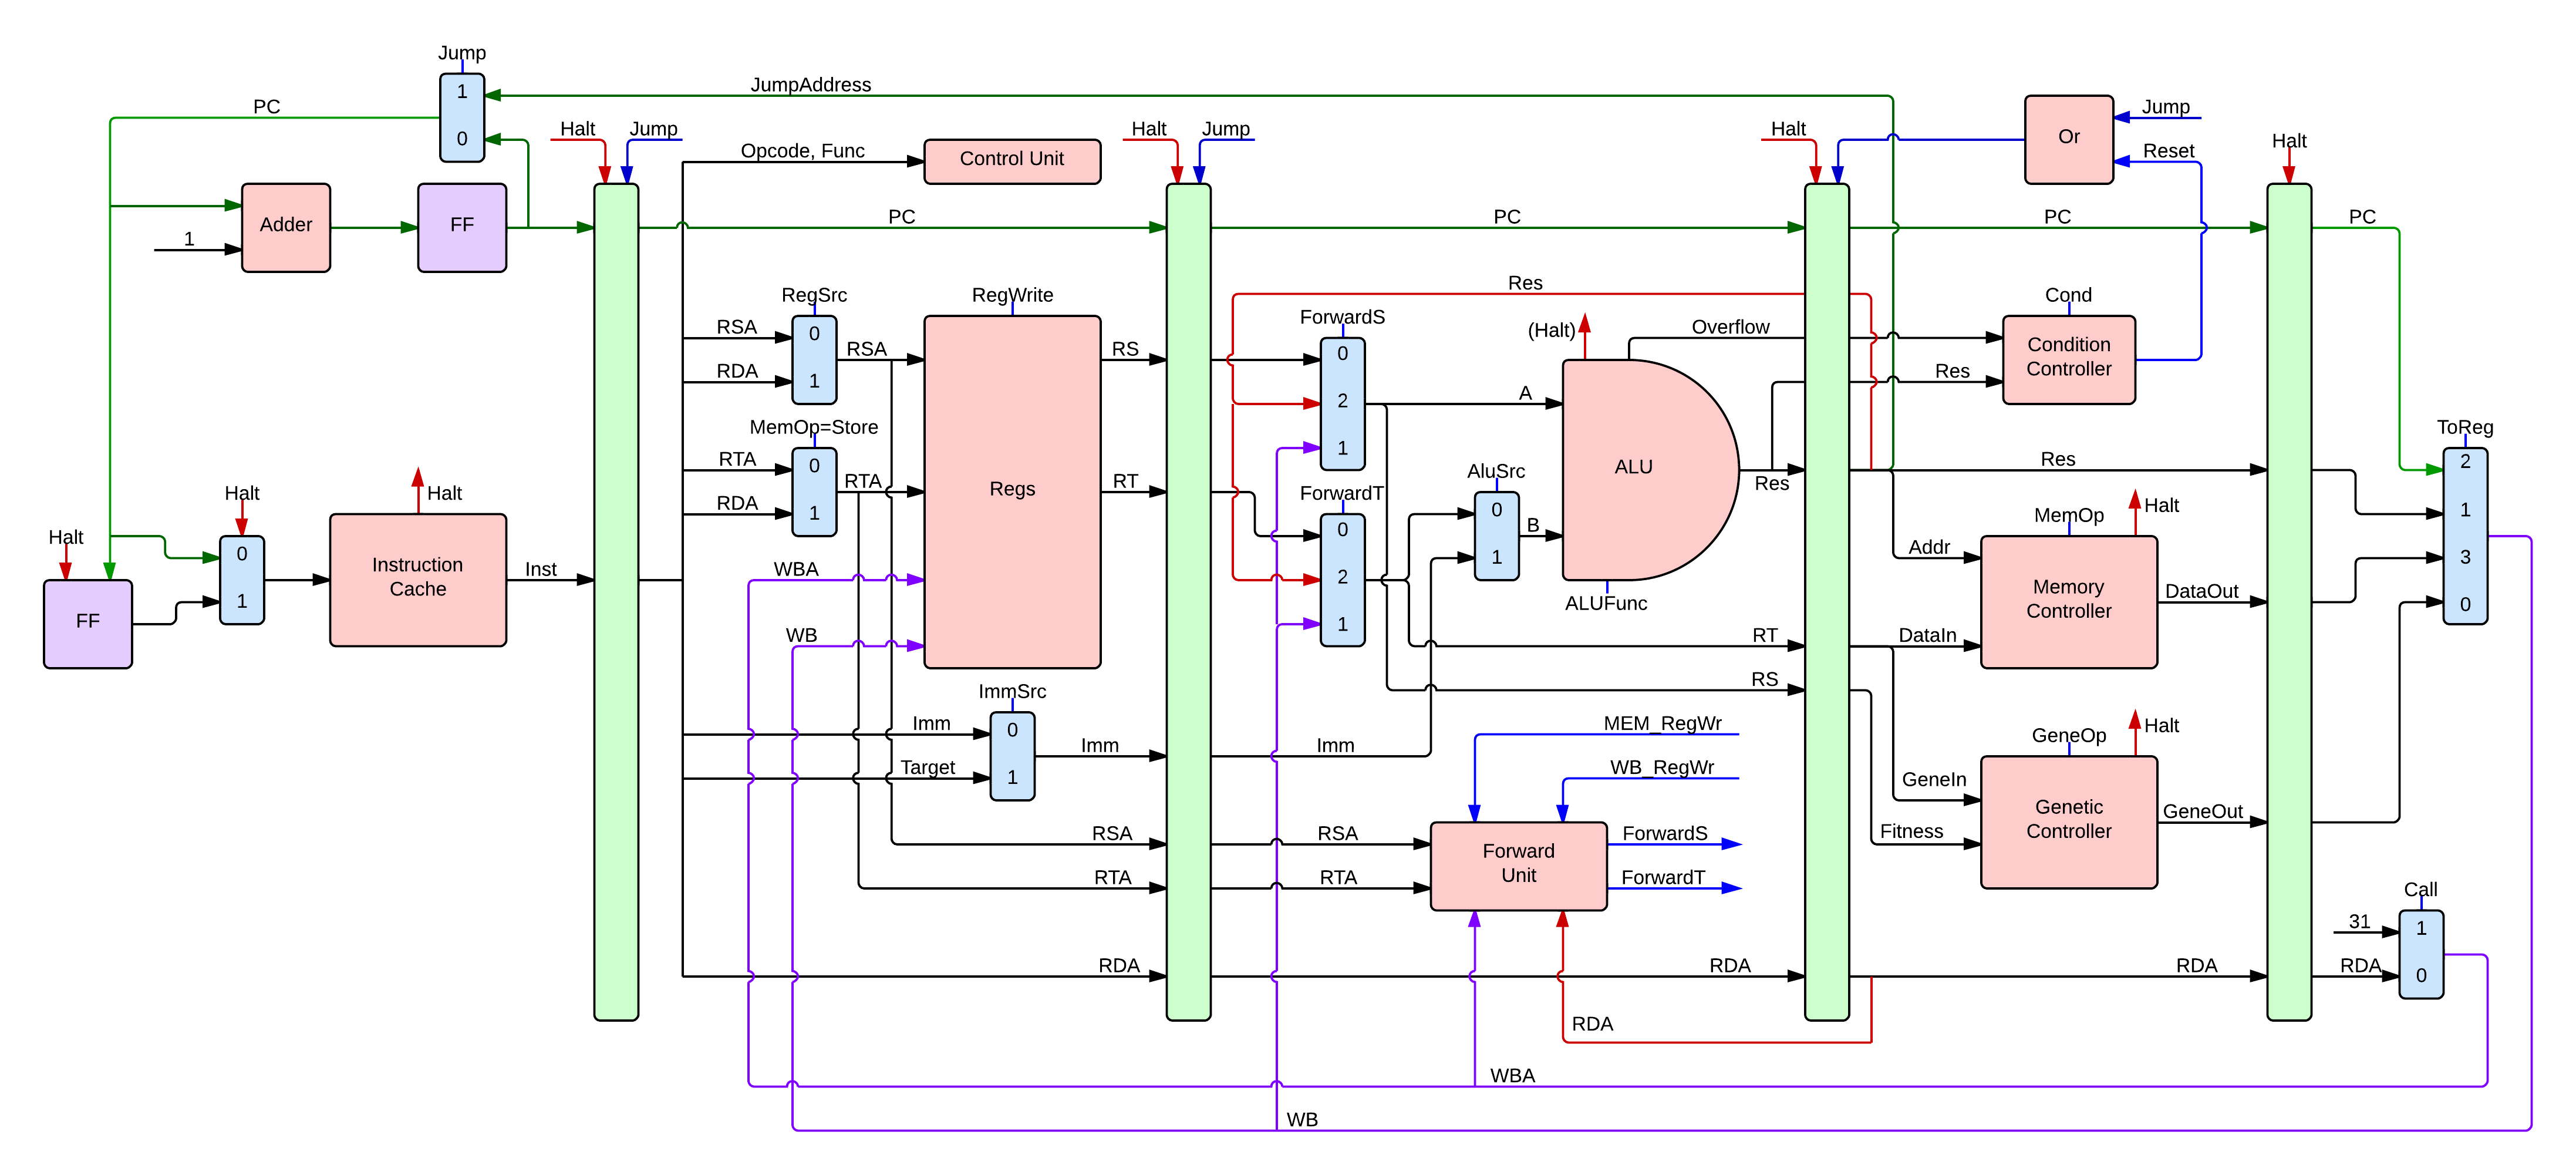
\includegraphics[width=\textwidth]{fpga/fig/fitness_core.png}
  \caption{Architecture block diagram}
  \label{fpga:fig:fitness:fitness_arch}
\end{figure}
.

The data path is simple.
The instruction is the same length for all the instructions.
This makes it easier to fetch the instruction in the first stage and decode it in the second.
Also, the ISA only supports three different instructions classes with the register mappings located on the same positions.
This allows the register file to be read on the same time as the control unit determines the correct control signals for that particular instruction.
This allows for a shorter pipeline.
If the instruction format where not symmetric, we would need to split the register file and decode stage in two stages.
A bigger pipeline would imply higher risk for pipeline hazards, and a more complicated hazard detection and correction schemes. 

The data path is in fact a load/store architecture.
This simplifies the execution and memory interaction.
Note that memory operands only appear in load and store instructions.
This implies that the execution stages is responsible for calculating the memory address and that the memory access can happen in the following stage.
Allowing the ALU to operate on operands in memory would expand the address stage, memory stage and the execution stage \cite[p.~335]{compOrgDes}.
The resulting architecture would involve a deeper pipeline. 


The MIPS inspired pipeline allows the design to be simple, but still powerful.
It  will increase performance by effectively increasing the instruction throughput.
Note that instruction throughput is an important metric because real applications execute millions of instructions \cite[p.~335]{compOrgDes}



More advanced features like branch prediction and instruction scheduling are not taken into consideration while designing the data path.
The group decided that the overall design should be as simple as possible.
Hazard and branching schemes are kept simple.
Hazards are resolved with the \emph{forwarding unit}, which forwards data if dependencies are detected.
Branching are resolved with use of \emph{conditional} codes in each instructions.
The reader may refer to their respective sections for more details.



\subsubsection{Control Unit} 
The responsibility of the control unit is to configure all the different components for the current CPU operation so that the desired computation will emerge from the flow of data.
The control unit achieves this by setting the control signals of the relevant control signals of the relevant components to the values associated with the current instruction.
Note that different instructions classes requires different use of the data path.
Thus, combinations the control signals must accommodate the different instructions formats. The different instructions classes and their control can be seen in table \ref{fpga:fitness:control_unit_out_tbl}. 

The control unit sets up the components based on the \emph{FUNCTION CODE} and the \emph{OPERATION CODE} of the instruction. The \emph{FUNCTION CODE} is the 4 least significant bits of the instruction, and is responsible for determining the operation the ALU should perform. 

 
\begin{table}
    \centering
    \begin{tabular}{| l | c | c | c |c |}
    \hline
    Control signals   &              &          &                   \\[0.5ex]
                      & RRR          & JUMP     &  SW   &  STG       \\
    \hline
    ALU\_SOURCE       &              &          &       &            \\
    IMM\_SOURCE       &              &          &       &            \\
    REG\_STORE        &              &          &       &            \\
    STORE\_SOURCE     &              &          &       &            \\
    CALL              &              &          &       &            \\
    JUMP              &              &          &       &            \\
    GENE\_OP          &              &          &       &            \\
    MEM\_OP           &              &          &       &            \\
    TO\_REG           &              &          &       &            \\
    \hline  
                      & RRI          & LW       & STI   & SETG       \\
    \hline
    ALU\_SOURCE       &              &          &       &            \\
    IMM\_SOURCE       &              &          &       &            \\
    REG\_STORE        &              &          &       &            \\
    STORE\_SOURCE     &              &          &       &            \\
    CALL              &              &          &       &            \\
    JUMP              &              &          &       &            \\
    GENE\_OP          &              &          &       &            \\
    MEM\_OP           &              &          &       &            \\
    TO\_REG           &              &          &       &            \\
    \hline
                      & CALL         & LDI      & LDG   &            \\
    \hline  
    ALU\_SOURCE       &              &          &       &            \\
    IMM\_SOURCE       &              &          &       &            \\
    REG\_STORE        &              &          &       &            \\
    STORE\_SOURCE     &              &          &       &            \\
    CALL              &              &          &       &            \\
    JUMP              &              &          &       &            \\
    GENE\_OP          &              &          &       &            \\
    MEM\_OP           &              &          &       &            \\
    TO\_REG           &              &          &       &            \\   
    \hline
    \end{tabular}
    \caption{Control unit output}
    \label{fpga:fitness:control_unit_out_tbl}

\end{table}

 


\begin{table}[h]
    \centering
    \begin{tabular}{| l | l |}
    \hline
    Opcode & Instruction class \\
    \hline
    1000   & RRR               \\
    1100   & RRI               \\
    0000   & LW                \\
    0001   & SW                \\
    0100   & LDI               \\
    0010   & JMP               \\
    0011   & CALL              \\
    0101   & STI               \\
    1001   & LDG               \\
    1010   & SETG              \\
    1011   & STG               \\
    \hline       
    
    \end{tabular}
    \caption{Overview of opcodes}
    \label{fpga:tbl:opcode_tbl}

\end{table}



\input{fpga/tbl/fitness_core_control_unit_tbl}


%%The meaning of the different control signals

The following paragraphs document and explain each of the control unit's control signals that control the functionality in the fitness core.

\paragraph{ALU\_FUNC}
The \emph{ALU\_FUNC} is the least four significant bits of the instruction, and is responsible for determining the type of operation the \emph{ALU} should perform. This are set according to table \ref{fpga:tbl:alu_function_codes_tbl} 

\begin{savenotes}
\begin{table}
\centering
    \begin{tabular}{| l | l |}
     \hline
     FUNC code & operation \\
     0000      & ADD       \\
     0001      & SUB       \\
     0010      & MUL       \\
     0011      & SRA       \\
     0100      & OR        \\
     0101      & AND       \\
     0110      & XOR       \\
     0111      & SLL       \\
     1000      & SRL       \\
     1001      & OP1 \footnote{Gives input 1 as output.}       \\
     1010      & OP2 \footnote{Gives input 2 as output.}      \\
     1111      & NOP       \\
     \hline
   \end{tabular}
    \caption{Overview of function codes}
    \label{fpga:tbl:alu_function_codes_tbl}



\end{table}
\end{savenotes}


\paragraph{ALU\_SOURCE}
The \emph{ALU\_SOURCE} signal is used to specify the second \emph{ALU operand}. When this signal is asserted the second ALU operand is the immediate field of the instruction. This implies that the instruction class of the instruction is either RRI or RI. On the other hand, if this signal is de-asserted, the operand comes from read register to of the instruction file. Note that this value may or may not have been forwarded. 

\paragraph{REG\_WRITE}
This signals specifies whether the value, residing in the \emph{write-back} stage, should be written to the register file. When this signal is asserted the value from the \emph{write-back} stage is written to the specified register address. The register address is specified in the instruction, and always reside in the RT address field of the instruction. This fact makes it simpler when deciding at what address the value should be written. However, when this signal is de-asserted, this is equivalent with no operation. 

\paragraph{IMM\_SOURCE}
The galapagos ISA have two different instruction classes (RI, RRI) that uses different lengths of the immediate field. In order to differentiated between these immediate fields, the \emph{IMM\_SOURCE} signal is responsible of selecting immediate field based on the instruction class of the current instruction. The selection is done with a multiplexor. In case of an RRI instruction the 10-bits immediate field is selected, and the 19-bits for a RI instruction.   


\paragraph{REG\_SOURCE}
In case of \emph{JMP} and \emph{CALL} instructions the immediate address field of the instruction is added with the address content of RD. The RD address specified in the in the instruction must be read from the register file. Normally, the register file would use the \emph{RS} and \emph{RT} part of the instructions as inputs to the register file. In the special case of \emph{RI} instructions the register file must read the RD instead of RS. This is accomplished by asserting the \emph{REG\_SOURCE} signal. This signals causes the a multiplexor to choose the \emph{RD} portion of the instruction instead of the \emph{RS} as input to the register file. This will output the content of the correct data from the register file. This is also visible in figure \todo{reference figure}   


\paragraph{STORE\_SOURCE}





\todo{this}

\paragraph{JUMP}
The jump instruction is use the address in the immediate field of the instruction to load a new value into the \emph{program counter} register. Which specifies the address of the next instruction to be executed. The jump signal is used in a multiplexor in the memory stage to select between the jump address or the incremented program counter. In case of jump, this signal is asserted and the jump address is chosen. When de-asserted the program counter is the incremented program counter. This signal is also asserted when performing call instructions which is discussed in the section below.   

\paragraph{CALL}
MIPS operate with what is known as a \emph{link-and-jump} instruction in order to support function calls \cn. The galapagos ISA also support this functionality, however, the instruction is denoted as \emph{CALL} instead of \emph{JAL}. The instruction works very similar to the jump instruction described above. The difference lay in the fact that the incremented program counter is stored in combination with the program counter being modified. This address is stored in register 31.This value can be used later when returning from the function call. The return of a function is basically a jump instruction that jumps back to the address after the call instruction.

The responsibility of the \emph{CALL} signal is to make sure that the incremented program counter is stored at register 31. When asserted the signal make sure that the write register address is changed to 31. If the signal is de-asserted the write register will stay unmodified, and the RT register in the instruction is responsible for specifying the register address.


\paragraph{GENE\_OP}
The loading and storing fitness values and chromosomes is the responsibility of the \emph{genetic controller}. This controller is able to perform three types of actions: \emph{load}, \emph{store} and \emph{settings} dependent of the instruction class executed. When performing a load, a chromosome is loaded from the unrated pool. The store operation is used to store a chromosome and its corresponding fitness value to the rated pool. The settings are used to apply settings to the genetic pipeline.  In order to divide these cases, the galapagos architecture rely on \emph{gene operation} vector. The bit-vector is set depending on the instruction class as seen in table \ref{fpga:tbl:gene_op_code_tbl}



\begin{table}[h]
\centering
    \begin{tabular}{| l | l | l |}
     \hline
     Code  & Meaning      & Instruction class \\
     \hline
     00    & NOP          &   OTHER           \\
     01    & LOAD\_GENE   &   LDG             \\
     10    & STORE        &   STG             \\
     11    & SETTINGS     &   SETG            \\
    \hline
    \end{tabular}
    
    \caption{Gene operation codes}
    \label{fpga:tbl:gene_op_code_tbl}
    

\end{table}


Depending on the bit-vector-signal, the \emph{genetic controller} is able to perform the appropriate action. 

\todo{Fix} 

\paragraph{MEM\_OP}
As with the genetic controller, the memory controller must be able to distinguish between operations. In case of memory controller, these operations are loading and storing to/from the external memory. In same manner as with, the genetic controller, these signals are set according to the instruction class currently being executed. These can be seen in table \ref{fpga:tbl:mem_op_code_tbl}

\begin{table}[h]
\centering
    \begin{tabular}{| l | l | l |}
     \hline
     Code  & Meaning      & Instruction class \\
     \hline
     00    & NOP          &   OTHER          \\
     01    & LOAD\_DATA   &   LW             \\
     10    & STORE\_DATA  &   SW             \\
    \hline
    \end{tabular}
    
    \caption{Memory operation codes}
    \label{fpga:tbl:mem_op_code_tbl}
    

\end{table}



\paragraph{TO\_REG}
In the \emph{write-back} stage, there is need to distinguish between several outputs from the \emph{memory stage}. The \emph{TO\_REG} signal is responsible for selecting which value that should be written to the register file. The selection is aided by a 4-to-1 multiplexor. The different inputs are: \emph{Gene}, \emph{Data}, and \emph{PC+1}, \emph{Res}, as seen in figure \todo{add reference}. However, keep in mind that the \emph{REG\_WRITE} signals must be asserted for the data to be written. 

The \emph{TO\_REG} bit-vector are set according to table \ref{fpga:tbl:to_reg_multiplexor_output_tbl}

\begin{savenotes}
\begin{table}[h]
\centering
    \begin{tabular}{| l | l | l |}
     \hline
     Code  & Output       & Instruction class \\
     \hline
     00    & GENE      &   LDG                \\
     01    & RES       &   OTHER \footnote{OTHERS refers to instructions that store the ALU result to a register }             \\
     10    & PC+1      &   CALL              \\
     11    & DATA      &   LW                \\
    \hline
    \end{tabular}
    
    \caption{4-to-1 multiplexor output}
    \label{fpga:tbl:to_reg_multiplexor_output_tbl}
    

\end{table}
\end{savenotes}


\subsection{The ALU}


\subsubsection{Multiplication}
Multiplication is handled as a special case in the architecture. The multiplication is designed to use two cycles in the \emph{execution stage}. This is because the multiplication is the slowest of the ALU operations, and the overall performance would be degrade if this case was treated as the longest path. To overcome this limitation, a state machine is designed in the execution stage to halt the pipeline when performing multiplication. This will make sure the multiplication operation is able to finish without needing to adjust the clock for the other arithmetic operations performed by the ALU. This will make the architecture to be able to run at greater clock speeds. 


\todo{fix this brain dump}



\subsubsection{Forwarding Unit} \label{fpga:fitness:sss:forwarding_unit}
Since the executions of instructions overlap in the pipeline.
There is need for some mechanism to handle the data dependencies that arise between the instructions. These dependencies are known as data hazards. They occur when a planned execution of an instruction cannot happen in that cycle because some data is not yet available. This problem can be solved in two ways, either by stalling or forwarding. Stalling, the simplest solution, is done by avoiding the hazard by stalling until the data becomes available. This is accomplished by inserting \emph{NOPs} in the pipeline. Although, this method work, it is to slow in most cases. Since this processor aim to achieve high performance this solution is far from optional. A far better approach is to rely on forwarding, also known as register forwarding. In this approach the aim is to resolve the dependencies by simply forwarding internal resources from other stages in the pipeline, if needed.

The forwarding logic is implemented by comparing register dependencies of the instruction in the execution stage with other instructions currently residing in the pipeline. If the forwarding unit notices register dependencies and that these instructions will write to these registers at a later time, it will assert signals that causes the data to be forwarded to the execution stage. The control signals is used in two 3-to-1 multiplexors in order to choose which source the data should arrive from. An overview of the control signals and their meaning can be seen in table. \ref{tbl:fpga:forwarding_signals}.

\todo{Perhaps this can be rewritten a bit}


\begin{table}[H]
    \centering
    \begin{tabular}{| p{2.5cm} p{9cm} |}
    \hline
    Control signal  & Meaning \\ [0.5ex]
    \hline 
    forwardA=00  & The first ALU operand is from the register file\\
    
    forwardA=10  & The first ALU operand is from the prior ALU result\\
    
    forwardA=01  & The first ALU operand is either data from memory or an earlier ALU      result\\
    
    & \\
    forwardB=00  & The second ALU operand is from the register file\\
    forwardB=10  & The second ALU operand is from the prior ALU result \\
    forwardB=01 & The second ALU operand is either data from memory or an earlier ALU result \\
    \hline
    \end{tabular}
    \caption{Forwarding control signals}
    \label{tbl:fpga:forwarding_signals}

\end{table}




\subsubsection{Conditionals} 
Like ARM , the galapagos architecture use conditional codes in order to determine if an instruction should be executed or not. Instead of using explicit branch instructions each instruction carries a 4-bit conditional code. Every instruction is in fact executed, however, the effect of the instruction is determined by the \emph{condition unit}. The \emph{condition unit} is implemented by checking the condition code of the current instruction against the status flags of the previous instruction. Dependent on this information the \emph{condition unit} produces an \emph{execute signal}. This signal is used to either, invalidate or approve the current instruction. However, this may also alter instruction stream and cause more instructions to be invalidated. Note that the determination of the branch is performed during the memory stage. This implies that the instructions following the branch is loaded in the pipeline. If the branch is not taken, this does not impose a problem since the instruction were going to be validated anyway. However, if the branch is taken, the instructions currently residing in the pipeline are not supposed to be validated. More specific, the instructions residing in the \emph{fetch stage}, \emph{decode stage}, \emph{execute stage} needs to be flushed.  This is accomplished with a 2-bit counter. The counter is used to determine how many instructions should be flushed when reaching the memory stage. Fortunately, this number is always three in case of a conditional branch.The instructions themselves are simply invalidated by invalidate their control signals. Note that the state is not changed until the memory stage and the write back stage. By simply intercept and change this signals the result of the instruction would in effect be a \emph{NOP}. 


\todo{reference}.

\todo{Better flow}



\subsubsection{Fitness Memory Controller} 
In order to communicate with the main data controller, each fitness cores contains a small version of the data controller to synchronise the communication to the main controller. This small controller, referred to as the \emph{fitness data memory controller}. The controller is implemented as a state machine, and is responsible for requesting the memory bus, and specify the type of operation the \emph{Data memory controller} is to perform on behalf of the \emph{fitness core}.  





Depending on the instruction, either load or store, the controller react by 

The \emph{fitness core} supports two instructions for interacting with the data memory,  \emph{load word} and \emph{store word}. 







To accommodate these instructions the memory controller have two cases, one for loading and one for storing a memory word, both which requires access to the bus. The \emph{fitness memory controller} requests the bus by sending a request signal to the main \emph{Data controller}. The \emph{Data controller} either a responds to this request, immediately granting the bus with an acknowledgment, or prosponds sending acknowledgment, in case some other core is using the bus. Either way, the requesting fitness core will halt the pipeline waiting for access to the bus. 

When the bus is acquired, the \emph{fitness memory controller} puts the address on the address bus. Depending on the operation, \emph{LOAD} or \emph{STORE}, it either receives data on the input bus, or puts data on the output bus. 




\subsubsection{Fitness Genetic Controller} 
As with the communication with the main data controller, each fitness core also have a small controller to synchronise the communication with the \emph{genetic memory controller}. This controller is referred to as the \emph{fitness genetic controller}. This controller is also implemented as a state machine. However, this component contains more functionality than the \emph{fitness memory controller}. The communication against the genetic controller require more functionality, since this controller communicate with the \emph{genetic controller}, which handles the access with both the rated and unrated pool. 





\subsubsection{Halting the pipeline}
In normal computer systems the time to access the memory is variable. It depends on the different states of the machine. This imposes a problem when several cores competes about access to the memory. It is difficult to determine precisely the times that is actually used to receive the required data. In order to fix this issue, and prevent the processor to compute when there is no data. Each interaction with memory is able to halt the processor in case when performing memory operations. The different situations arise when accessing the instruction memory, data memory, and the genetic data pools. Their corresponding controllers are able to set a halt signal before performing the operation. When the \emph{halt} signals is asserted, the program counter and the pipeline registers will be halted, ensuring that the \emph{fitness core} does not change state. 

\todo{hmm? Integrate with the controllers} 




